% !TeX root = markov.tex

\section{The Ehrenfest model}\label{s.ehrenfest}

\textbf{Problem} The Ehrenfest model is designed to model diffusion of particles between two containers. In the following diagram there are four particles in the left container and six particles in the right container for a total of $n=10$ particles:
\begin{center}
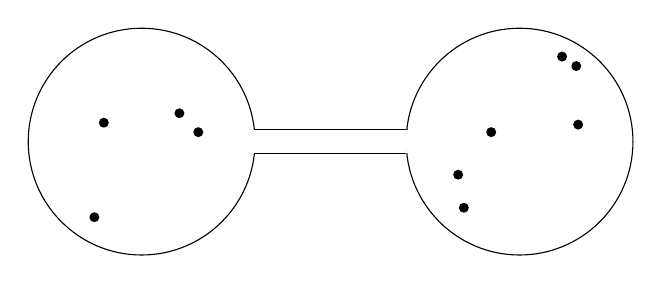
\begin{tikzpicture}[scale=1.2]
\draw (0,0) node {} circle[radius=1.2];
\draw[white,thick] (-6:1.2) arc(-6:6:1.2);
\draw (-6:1.2) -- +(1.63,0);
\draw (6:1.2) -- +(1.63,0);
\fill (-.4,.2) circle[radius=1.5pt];
\fill (.4,.3) circle[radius=1.5pt];
\fill (-.5,-.8) circle[radius=1.5pt];
\fill (.6,.1) circle[radius=1.5pt];
\begin{scope}[xshift=4cm]
\draw (0,0) node {} circle[radius=1.2];
\draw[white,thick] (174:1.2) arc(174:186:1.2);
\fill (-.3,.1) circle[radius=1.5pt];
\fill (.45,.9) circle[radius=1.5pt];
\fill (-.65,-.35) circle[radius=1.5pt];
\fill (.62,.18) circle[radius=1.5pt];
\fill (-.59,-.7) circle[radius=1.5pt];
\fill (.6,.8) circle[radius=1.5pt];
\end{scope}
\end{tikzpicture}
\end{center}
Repeated choose a particle at random with uniform distribution and move it to the other container. If there are $i$ particles in the left container then the probability of choosing a particle from the left container is $i/n$ and the probability of choosing a particle from the right container is $(n-i)/n$. If one container is empty the next particle must be chosen from the other container. 

The problem is similar to the gambler's ruin except that: (a) the process never ends and (b) the probability of a left or right step changes with each step:
\begin{center}
\begin{tikzpicture}[scale=1.2]
\draw (0,0) node[above left] {$A$} -- 
      (10,0) node[above right] {$B$};
\foreach \x in {0,1,2,3,4,5,6,7,8,9,10} {
  \draw (\x,0) -- +(0,4pt);
  \node at (\x,-10pt) { $\x$ };
}
\node at (4,-9mm) {$i$};
\node at (10,-9mm) {$n$};
\draw[fill] (4,7mm) circle[radius=1pt];
\draw[->] (4,7mm) -- node[above,xshift=-8pt] {$(n-i)/n$} +(-1,0);
\draw[->] (4,7mm) -- node[above,xshift=2pt] {$i/n$} +(1,0);
\draw[->] (0,7mm) -- node[above] {$1$} +(1,0);
\draw[<-] (9,7mm) -- node[above] {$1$} +(1,0);
\end{tikzpicture}
\end{center}

\subsection{Theoretical results}

The process is a Markov chain which eventually reaches a \emph{stationary distribution}:
\[
s_i=\dischoose{n}{i}\left(\frac{1}{n}\right)^n\,,
\]
where $s_i$ is the proportion of time that the particle is at the $i$'th position.

\subsection{Running the simulations}

The program asks the user how to run the simulation: with the saved value of $n$ or with a new value of $n$. Here is an output of the simulation:
\begin{verbatim}
Total particles in urns = 10
Theoretical stationary distribution
[0.001 0.01  0.044 0.117 0.205 0.246 0.205 0.117 0.044 0.01  0.001]
Simulation stationary distribution
[0.001 0.009 0.044 0.12  0.208 0.243 0.205 0.121 0.042 0.008 0.001]
\end{verbatim}
A graph of these distributions is shown in Figure~\ref{f.ehrenfest1}; the theoretical distribution and the result of simulation are so close together that the lines are slightly offset.

\begin{figure}
\begin{center}
\includegraphics[width=\textwidth]{ehrenfest-01}
\caption{Stationary distribution for the Ehrenfest model}\label{f.ehrenfest1}
\end{center}
\end{figure}

